% This chapter should describe what was actually produced: the programs which were written, the hardware which was built or the theory which was developed. Any design strategies that looked ahead to the testing stage should be described in order to demonstrate a professional approach was taken.

% The repository overview should be around one page in length and should describe the high-level structure of the source code found in your source code repository. It should describe whether the code was written from scratch or if it built on an existing project or tutorial.

% Contribution to the field, with genuine potential for impact outside the tripos.

% Challenging goals and substantial deliverables, all methods and tools deployed expertly.

% Original techniques or methodologies going beyond what was previously known.

% Presentation is clear and concise throughout, with creative use of figures or diagrams.

% Excellent repository overview, giving clear insight into project structure.

\label{sec:3}

\section{Agent Architectural Overview}
\label{sec:architectural-overview}

\begin{figure}[h]
    \centering
    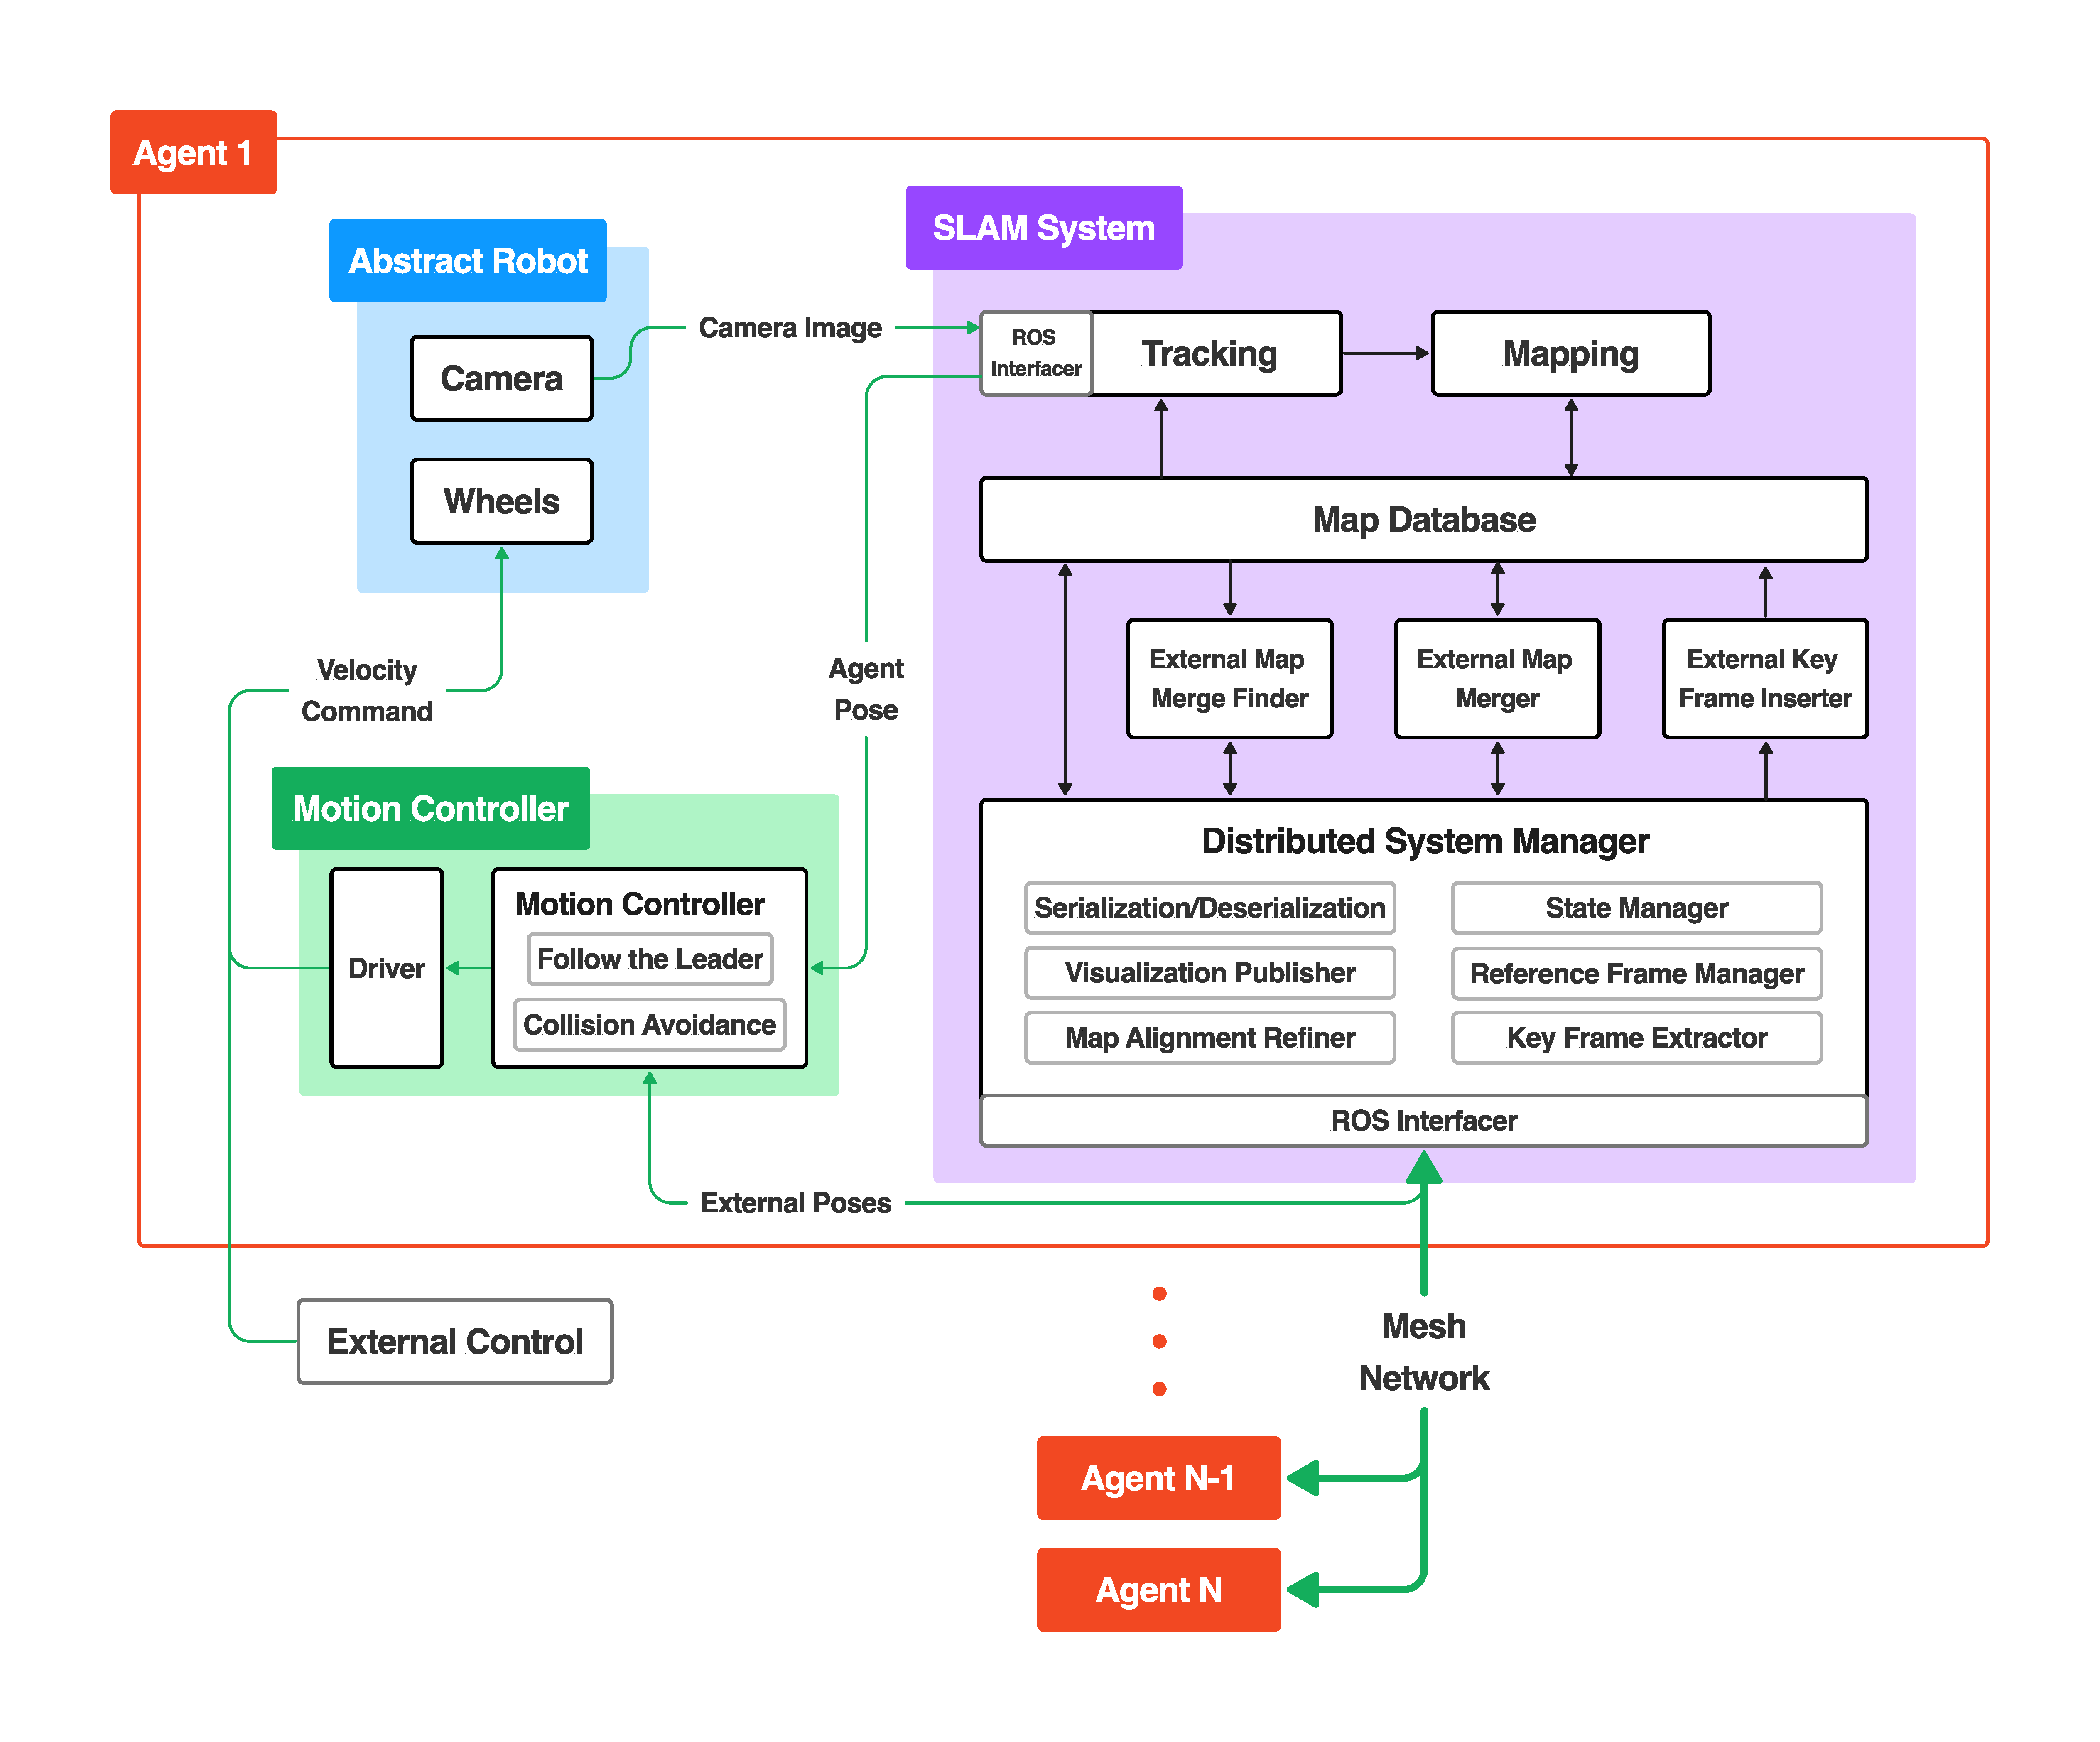
\includegraphics[trim=5cm 5cm 5cm 5cm, scale=0.2]{figures/agent_diagram.pdf}
    \caption{Agent diagram. Green arrows represent messages sent over ROS topics, while black arrows are internal communications within a node.}
    \label{fig:agent-diagram}
\end{figure}

\autoref{fig:agent-diagram} gives an architectural overview of an agent, showing how the \texttt{Abstract Robot}, \texttt{SLAM System} and \texttt{Motion Controller} ROS nodes interconnect.

From a high level, we have an \texttt{Abstract Robot} node that provides an interface to the robot's hardware, as explained in \autoref{sec:ros-2}. This sends camera images to the \texttt{SLAM System} node, which builds a map of the world in collaboration with its peers. The \texttt{Motion Controller} node receives agent pose information from both the local \texttt{SLAM System} and the external peers to perform tasks such as collision avoidance by sending velocity commands back to the \texttt{Abstract Robot} node, closing the control loop.

In the following sections, we will explore these nodes in detail.

\section{SLAM System}
\label{sec:slam-system}
The SLAM System node is the majority of this project's implementation. It processes monocular images from the camera to localize the agent while also collaboratively building up a map of the world with its peers. As discussed in \autoref{sec:starting-point}, my system is based on an existing single-agent SLAM system that performs the \texttt{Tracking} and \texttt{Mapping} tasks. While substantial modifications were made to the base single-agent system, I will generally focus on the decentralized layer I have built on top in the interest of space.

TODO: Add info on map datastructure

\subsection{Decentralized System Manager}
\label{sec:decentralized-system-manager}
Decentralized collaborative SLAM systems have significantly more complexity than a single-agent or even centralized collaborative system, due to the complex interactions between agents as they merge maps, lose localization, or lose connection with the network. Therefore, a robust framework must be put in place to ensure the robustness and corectness of the system, which I have implemented in the \texttt{Decentralized System Manager} component.

For the sake of simplicity, the following explanations will explore the interactions between just two agents: a \textit{local} and \textit{external} agent. In the \textit{\nameref{sec:generalizing-to-n-geq-3-agent-systems}} Section, we sill show how this easily generalizes to a system with an arbitrary number of agents when augmented by some simple rules.

\subsubsection{State Manager}
\label{sec:state-manager}

\begin{figure}[h]
    \centering
    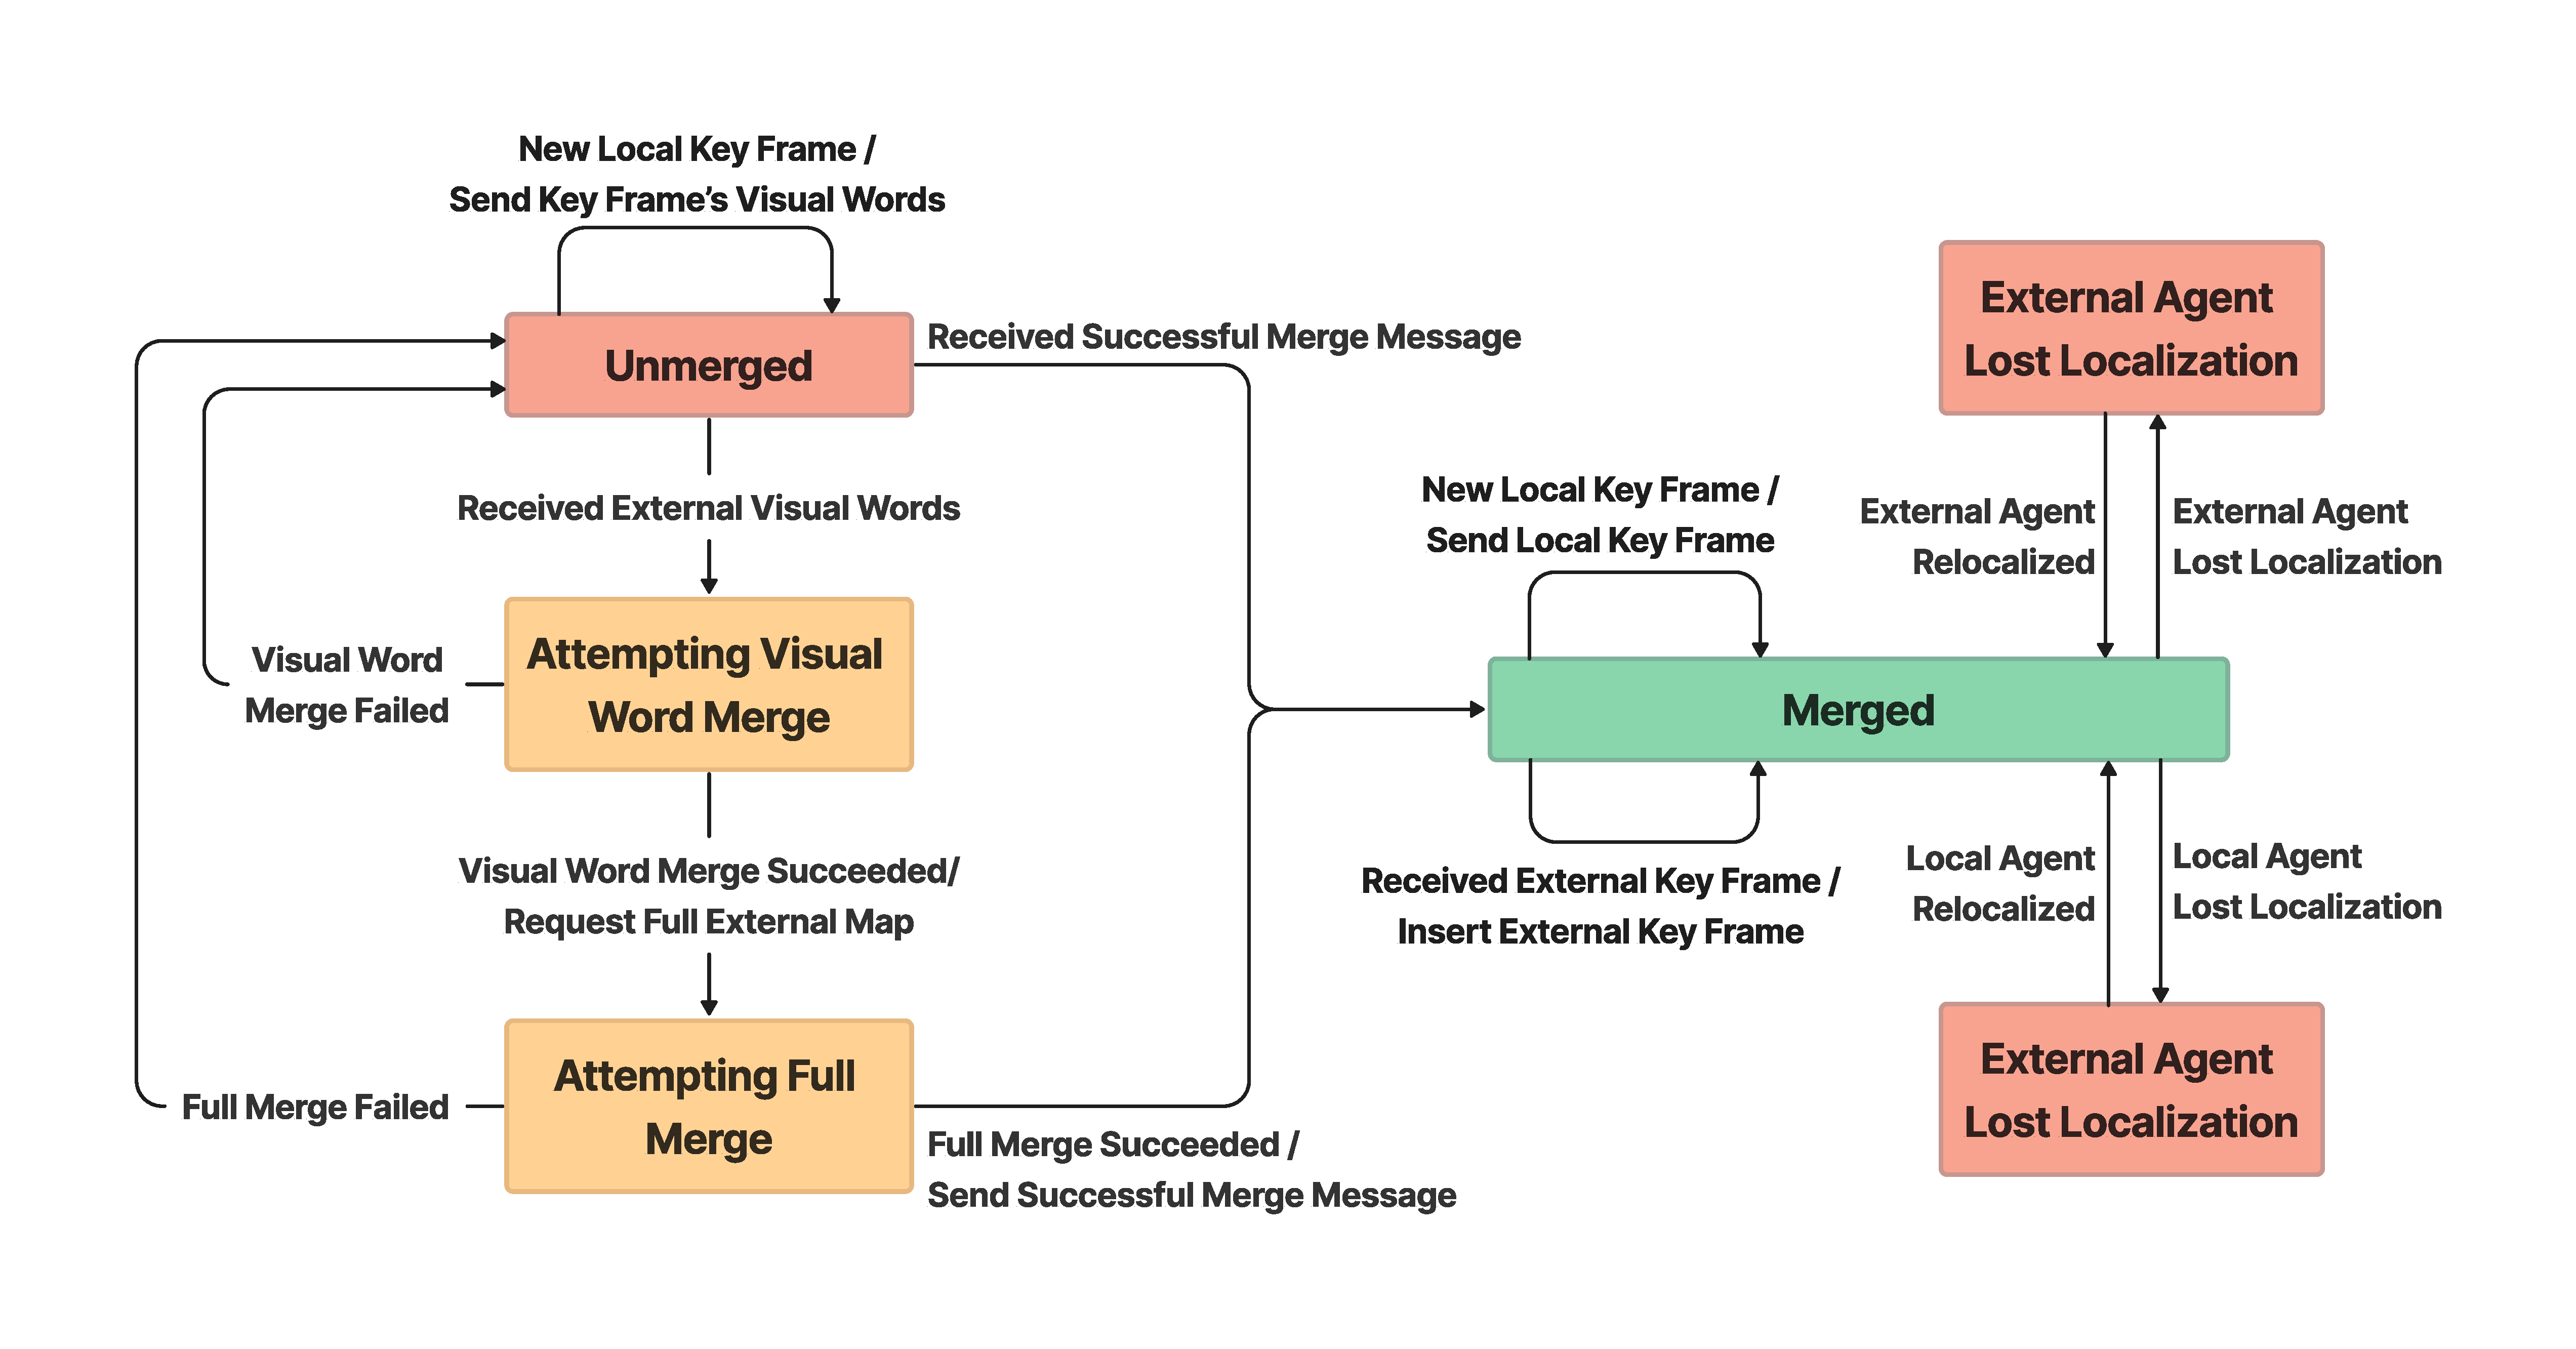
\includegraphics[trim=5cm 5cm 5cm 5cm, scale=0.2]{figures/slam_system_state_machine.pdf}
    \caption{SLAM system state machine for a single peer.}
    \label{fig:state-machine}
\end{figure}

Each agent's \texttt{Decentralized System Manager} maintains a state machine for every peer in the system, shown in \autoref{fig:state-machine}. All peers are initially in the \texttt{unmerged} state, meaning that they are in different coordinate frames and can not collaboratively build a map together. As the local agent starts to explore the same places as its peers, we are able to recognize the visual overlaps and merge their maps, bringing us to the \texttt{merged} state where the agents share the same coordinate frame and map, enabling relative positioning and collaborative map building.

\subsubsection{External Map Merge Finder}
\label{sec:external-map-merge-finder}
A naive approach to merging maps with an external agent is to constantly exchange our full maps, each time trying to identify if a map merge is possible. While simple, this approach clearly does not scale well from both a networking and computational perspective, as maps are often \>1MB in size and computing a full map merge is extremely computationally expensive.

Instead, we first identify if a map merge is even feasible by using visual words before attempting a full map merge. This eliminates superfluous map merge attempts that have no chance of succeeding because the agents' maps have no visual overlap.

As the agents generate new key frames, we calculate the \hyperref[sec:visual-bag-of-words]{visual bag of words} seen by that key frame and send them to our peers over the \texttt{/new\_key\_frame\_bows} ROS topic. These visual words are significantly smaller than sending over the complete map and enable agents to detect if there is a significant amount of visual overlap between its local map and the external agent's map. This is computed by \autoref{alg:map-merge-finder}.

This method gives a recall of almost 100\%, at the cost of potentially lower precision. This is a worthwhile tradeoff however, as it is essential to have very few false negatives so we can merge maps as soon as possible so the agents can begin collaborating and determine relative positioning. TODO: generate stats on this?

TODO: generate stats on how much this cuts down on bandwidth and computation

\begin{algorithm}
    \caption{Map merge finder using visual words. TODO: improve}
    \label{alg:map-merge-finder}
    \begin{algorithmic}[1]
        \Require{$E$: Set containing external key frame's visual words}
        \Ensure{$success$: Boolean value signaling if a merge is possible based on visual words}
        \State $(externalMergeScore,\ bestMatchKeyFrame) \gets CalculateMergeScore(E)$
        \State $I \gets ComputeVisualWords(bestMatchKeyFrame)$
        \State $(internalMergeScore,\ _) \gets CalculateMergeScore(I)$
        \State $success \gets externalMergeScore \geq internalMergeScore$
    \end{algorithmic}
\end{algorithm}

\subsubsection{External Map Merger}
\label{sec:external-map-merger}
Once a potential map merge with the external agent is identified by the \hyperref[sec:external-map-merge-finder]{external map merge finder}, we can begin a full merge attempt. We first request the full map from the external agent through the \texttt{/get\_current\_map} ROS topic. Once the map is received, we deserialize it and place it into our \textit{map database} data structure.

From this point, we need to confirm that a map merge is possible using the full map data.

TODO

Given the external key frame $k_0$ whose visual words triggered this map merge attempt, we extract a \textit{local window} $K$ of key frames connected to $k_0$ in the covisibility graph.

If the full map merge is ultimately successful, we broadcast a \texttt{/successfully\_merged} message to tell the external agent that we have successfully merged their map. The external agent will then move to the \texttt{merged} state and both agents will begin sharing key frames with each other.

It is important to note that this system requires only one agent to calculate the map merge, significantly reducing the computational overhead of map merging, especially in systems with many agents (further explained in \autoref{sec:generalizing-to-n-geq-3-agent-systems}).

\subsubsection{Keeping Maps Merged}

\subsubsection{External Key Frame Inserter}
\label{sec:external-key-frame-inserter}
Once the local and external agents have merged their maps and share the same coordinate frame, they can begin sharing key frames with each other.

Each agent maintains a set of sent key frames $K_{sent}$ and map points $M_{sent}$. The set of unsent key frames and map points are therefore represented as $K_{unsent} = K / K_{sent}$ and $M_{unsent} = M / M_{sent}$ respectively. Once $\#K_{unsent}$ exceeds a certain threshold, we serialize $K_{unsent}$ and $M_{unsent}$ and send them to the external agent. Finally, we add $K_{unsent}$ to $K_{sent}$ and $M_{unsent}$ to $M_{sent}$

Upon receiving the serialized key frames and map points, the external agent deserializes them and adds them to a queue to await insertion into their local copy of the shared map by the \textit{external key frame inserter}.

The external key frame inserter is run whenever we have spare cycles on the CPU, to prevent impacting the local tracking and mapping performance. The insertion process involves the following operations:

\begin{enumerate}
    \item \textbf{Pop external key frame $k_{ext}$ from front of queue}.
    \item \textbf{Relink $k_{ext}$ with covisible key frames and observed map points in the local map}. \\
          $k_{ext}$ contains references to its covisible keyframes and child map points that have already been sent or were generated by another agent. We search our local map for objects that match these references, reconnecting them. More details of the deserialization process are given in \autoref{sec:map-serialization-and-deserialization}.
    \item \textbf{Move $k_{ext}$ and its new external observed map points $M_{ext}$ to the local map}.
          Since the local and external agents are merged and in the same coordinate frame, we can simply move $k_{ext}$ and $M_{ext}$ to our local map without any transformations.\footnote[1]{I had previously used a \textit{key frame anchor} method, where instead of $k_{ext}$ having an absolute pose we would send its pose relative to the previous $k_{ext}$. The thought process behind this was to prevent minor misalignments between the local and external maps from preventing external key frames from properly integrating with the local map. However, experimental testing showed that this method instead caused the local and external maps to frequently diverge.}
    \item \textbf{Relink $M_{ext}$ with key frames in the local map which observe it}. \\
          $M_{ext}$ contains references to key frames which observe it which have already been sent or were generated by another agent. We search our local map for key frames that match these references, reconnecting them. More details of the deserialization process are given in \autoref{sec:map-serialization-and-deserialization}.
    \item \textbf{Merge $M_{ext}$ with map points in the local map}. \\
          $M_{ext}$ will already be correctly linked to observing key frames in the local map, however, due to communication latency some map points in $M_{ext}$ may be duplicates of existing map points in the local map. Therefore, we exploit spatial locality to combine duplicate map points that describe the same physical feature. A key observation was that this step is essential to ensuring the local and external keyframes stay well connected, ensuring the local and external maps do not diverge.

          TODO: add more details? idk
    \item \textbf{Perform a local bundle adjustment around $k_{ext}$}. \\
          Since we have merged map points in the previous step, we need to perform bundle adjustment to tweak the key frame and map point locations to minimize reprojection error. This helps create a more accurate map, minimizing tracking error. We also only need to perform this bundle adjustment locally, greatly reducing the computational cost.
\end{enumerate}

TODO: add diagram

\subsubsection{Local Key Frame Inserter}
\label{sec:local-key-frame-inserter}
As mentioned in the \nameref{sec:external-key-frame-inserter} section, it is essential that the local and external maps stay well connected, sharing the majority of their map points. In other words, we must use the external map points when running the 7 point algorithm (TODO: ref section?) to generate new local key frames.

The \textit{Tracking} and \textit{Mapping} modules, which are responsible for localizing the robot and generating new key frames, only interact with the \textit{Map Database}. Our external key frame inserter does all the work of properly reconecting external map points and merging duplicate map points, leaving the \textit{Map Database} datastructure looking as if all the map points and key frames were generated locally. This essentially abstracts the \textit{Tracking} and \textit{Mapping} modules away from the distributed aspects of the system, meaning they fully use the external map points when localizing the agent and generating new key frames.

\subsection{Generalizing to $N \geq 3$ Agent Systems}
\label{sec:generalizing-to-n-geq-3-agent-systems}
Now that we have explained how a pair of agents interact, we can explore how this can be generalized to a system with an arbitrary number of agents.

We assume a system with $N$ agents $A=\{agent_1, agent_2, ..., agent_N\}$, where $agnet_i$ is the agent with ID = i. Within this system we maintain a state $S_i=state_{n-m}$ for every agent pair $(agnet_n, agnet_m)$, giving us a total of $N(N-1)/2$ states. Conceptually, this is a fully connected graph with agents as the nodes and states between agents as the edges. We also have a set $G$ which contains all the groups of merged agents. The \textit{group leader} is defined as the agent in a group with the lowest agentId.

In the case where agents can lose communication with one another, we also assume that if any given $agent_n$ is able to communicate with an $agent_m$, $agent_n$ can also communicate with all of $agent_m$'s children. This is held if the agents are using a mesh network to communicate, for example.

Initially, every agent pair is unmerged so every state in $S$ is set as \textit{unmerged} and $G=\{\{agent_1\}, \{agnet_2\}, ..., \{agent_N\}\}$

A key insight of my distributed SLAM system is to delegate all merge operations to group leaders. This means that instead of all agents attempting merges with every other agent, only group agents have to attempt merges amongst themselves. This is significant, as the computational load of these merge operations scale proportional to the square of the number of agents involved, and in most use cases the number of group leaders quickly drops to be much lower than the total number of agents.

Additionally, having all merge operations performed by the group leader prevents potential race conditions introduced by communication latency within a group, for example two agents within a group both merging with different agents at the same time.

As discussed in the \hyperref[sec:external-map-merge-finder]{External Map Merge Finder} and \hyperref[sec:external-map-merger]{External Map Merger} Sections, the two major operations needed to merge are (1) exchanging visual words to identify visual overlap and therefore merge opportunities and (2) sending over the map and attempting a full map merge.

Tackling (1) first, instead of the group leader only sending the visual words of its own key frames, it will send the visual words of all key frames generated by agents within its group. Keep in mind that it will only be sending these visual words to other group leaders. This introduces no additional intra-group communication, as all agents within a group already send each other all new key frames.

Moving on to (2), once a pair of group leaders $(agnet_n, agnet_m)$ (with $n<m$) have successfully merged their maps, the agent with the larger ID ($agnet_m$) will change its coordinate frame to the agent with the smaller ID ($agent_n$). $agent_m$ will then send the transform from $agent_m$ to $agent_n$'s coordinate frame to the other agents in its group, allowing them to also change to $agent_n$'s coordinate frame. After this has been completed, $agent_m$'s group merges into $agent_n$'s group using \autoref{eq:1}, and agents begin exchanging key frames to update each other's maps. Eventually, once all agents are merged together, they will all be in $agent_0$'s coordinate frame.

Agents are able to keep track of the current groups and group leaders within the decentralized system since all successful merge messages are broadcast on the shared \texttt{/successfully\_merged} ROS topic.

TODO: fix obviously
\begin{gather} \label{eq:1}
    i \in G_n, j \in G_m, state_{i-j} \in S.\ state_{i-j} = merged\\ \text{where $G_n \in G$ and $G_m \in G$ are $agent_n$ and $agent_m$'s groups respectively.}
\end{gather}

This is perhaps best represented in visual form. Take the simple example where: ...



\subsubsection{Map Alignment Refiner}
\label{sec:map-alignment-refiner}
As our shared map grows, the maps stored locally by the agents may "fall out of alignment". By this, we mean that the maps are slightly translated, rotated, or scaled with respect to the lead agent's map TODO: define. This is largely a side effect of our aggressive early merge strategy which may merge two agents' maps before there is significant overlap, causing the estimated map alignment (ie. transformation between the two agents' origins) to have some error.

These small alignment errors are completely acceptable when maps are small, but may cause the maps to diverge as they grow.

To remedy this problem, we continuously refine our map alignment using \nameref{sec:ransac} and the Kabsch-Umeyama point alignment algorithm. After enough changes have been made to our local map, we perform the following steps:

\begin{enumerate}
    \item \textbf{Request map point locations from the lead agent}. \\
          This is defined as the set $TaggedMP_{ext}$ where ${TaggedMP_{ext}}_i = (uuid, (x, y, z))$
    \item \textbf{Extract local map point locations}. \\
          This is defined as the set $TaggedMP_{local}$ where ${TaggedMP_{local}}_i = (uuid, (x, y, z))$
    \item \textbf{Use the Kabsch-Umeyama and RANSAC algorithms to find transform $T$ which best aligns $TaggedMP_{ext}$ to $TaggedMP_{local}$.}
          The Kabsch-Umeyama algorithm finds the SIM(3) transformation $T$ from $TaggedMP_{ext}$ to $TaggedMP_{local}$, minimizing the RMSE. However, our input data has a large number of outliers so we use RANSAC on top to find a good fit while ignoring outliers.

          The RANSAC and Kabsch-Umeyama algorithms are described in detail in \autoref{sec:ransac} and \autoref{sec:kabsch-umeyama-algorithm} respectively.
    \item \textbf{Apply transformation $T$ to our local map.}
\end{enumerate}

\subsubsection{Reference Frame Manager}
\label{sec:reference-frame-manager}

\subsubsection{Visualization Publisher}
\label{sec:visualization-publisher}

\subsubsection{Losing Localization}
\label{sec:losing-localization}

\subsection{Map Serialization and Deserialization}
\label{sec:map-serialization-and-deserialization}
Map serialization and deserialization are essential and non-trivial components of this SLAM system, allowing agents to share their maps across the network. For this task, I used the Boost \autocite{boostLibrary} Serialization C++ library since it supports standard library collections and other common classes.

As discussed in \autoref{sec:slam-system}, maps contain key frames and map points. Individually, these objects are relatively easy to serialize with boost – in fact, the single agent SLAM program my system is based on already supported saving and loading maps allowing me to leverage some of their serialization helper functions. To serialize these objects we simply need to define a serialization scheme for each custom class, describing which class variables should be serialized and which shouldn't. Strategically selecting only the parameters that need to be serialized allows us to cut back on communication overhead. For example, there is no need for us to serialize a key frame's raw image, as it is not used in the rest of our SLAM pipeline.

Complexities arise when we try to serialize/deserialize the connections between these objects, especially when we are only sending map fragments. For example, if we send a new key frame $k$ and its map points $M_k$ to an external agent, due to the many-to-many relationship between key frames and map points, some of the map points in $M_k$ may have already been sent before. We can define $M_k = M_{k\_sent} \cup M_{k\_unsent}$, where $M_{k\_sent}$ are the map points that have already been sent to the external agent and $M_{k\_unsent}$ are the ones that have not. Map points in $M_{k\_sent}$ will need to be connected to $k$ when it is deserialized by the external agent, and map points in $M_{k\_unsent}$ will need to be sent to the external agent and connected to any existing keyframes in the external map that observe the map points.

We manage these connections by giving every key frame and map point a universal unique identifier (UUID), allowing us to use these UUIDs as references to a specific object in our multi-agent system. The beauty of UUIDs is that they do not require a centralized server to assign a unique ID to every object. Instead, we can generate the unique IDs without any communication with our peers\footnote[1]{While not \textit{verifiablly} unique, UUIDs are unique within practical limits. A commonly cited anecdote is that it is far more likely for a cosmic ray to cause a bug than a UUID collision.}.

TODO: add figure of this map fragment serialization and deserialization

This method of using UUIDs as references is used to rebuild all connections after deserialization, including the keyframe-to-keyframe connections that build the co-visibility graph and many others which I have not had the space to discuss in this dissertation.

\section{Motion Controller}
\label{sec:motion-controller}
While not a part of the core SLAM system, the motion controller node closes the control loop and demonstrates the real-world usability of my system. From a high level, the motion controller node consumes the local and external agents' poses and outputs a command velocity to the robot's movement system – all via ROS topics. For this project, I have implemented two different motion control systems which can be switched out seamlessly.

\subsection{Follow The Leader}
\label{sec:follow-the-leader}
The "follow the leader" motion controller consists of two agents: one leader and one follower. The follower is given a position and rotation offset to the leader which it attempts to maintain as the leader is moved around.

For example, you could set the follower to be 1 meter behind the leader and with a 180\textdegree{} rotational offset. This ensures that the leader and follower have no visual overlap, demonstrating that my SLAM system is truly building a shared map.

Spinning the agents around in a circle demonstrates that the two agents' maps are properly merged and that the agents are using map points generated by an external agent to localize themselves, giving accurate relative positioning even when there is no visual overlap at any given moment.

TODO: add figure of the map built

\subsection{Multi-Agent Collision Avoidance}
\label{sec:multi-agent-collision-avoidance}
The "multi-agent collision avoidance" example is more complex, employing a non-linear model predictive controller (NMPC) to avoid collisions with both static and dynamic obstacles. My NMPC system is derived from \autocite{DBLP:journals/corr/KamelASN17} and is defined as follows:

\subsubsection{Non-Linear Model Predictive Controller Formulation}
\label{sec:nmpc-implementation-details}
We assume an agent with current pose $\bm{p} \in \mathbb{R}^2$ and radius $r$. Firstly, we define our agent's control input $\bm{v_{cmd}}$ as a function describing its velocity over time. We can then define our agent's state $\bm{x}$ as the control input $\bm{v_{cmd}}$ applied to its current pose $\bm{p}$:

\begin{equation}
    \bm{x}(t) = \bm{p} + \int_{0}^{t} \bm{v_{cmd}}\ dt
\end{equation}

We can then solve the following minimization problem to find an optimal $\bm{v_{cmd}}$:
\begin{equation}
    \begin{aligned} \label{eq:nmpc-minimization-problem}
         & \min_{\bm{v_{cmd}}} \int_{t=0}^{T} J_x(\bm{x}(t), \bm{x_{ref}}(t)) + J_s(\bm{x}(t)) + J_d(\bm{x}(t))\ dt \\
         & \text{subject to } \bm{v_{min}} \leq \bm{v_{cmd}} \leq \bm{v_{max}}
    \end{aligned}
\end{equation}
where $T$ is our horizon length, $\bm{x_{ref}}$ is our target trajectory, and $J_x$, $J_s$, $J_d$ are the cost functions for this system.

Cost function $J_x$ rewards following the target trajectory $\bm{x_{ref}}$ and is shown below:
\begin{equation}
    J_x(\bm{x}, \bm{x_{ref}}) = \|\bm{x} - \bm{x_{ref}}\|^2
\end{equation}

$J_s$ and $J_d$ penalize collisions with static objects and dynamic objects respectively. They are defined as:
\begin{flalign}
    J_s(\bm{x}) & = \sum_{i=1}^{N_{static}} \frac{s_s*Q_s}{1 + \exp(d_i^{static} / s_s)}   \\
    J_d(\bm{x}) & = \sum_{i=1}^{N_{dynamic}} \frac{s_d*Q_d}{1 + \exp(d_i^{dynamic} / s_d)}
\end{flalign}
where $d_i^{static}$ is the distance between the agent and the $i-th$ static obstacle, and $d_i^{dynamic}$ is the distance between the agent and the $i-th$ dynamic obstacle. For example, if the $i-th$ dynamic obstacle is another agent with radius $r$ then $d_i^{dynamic} = \|\bm{x}(t)-\bm{x_i}(t)\|^2 - r$. $Q_s>0$ and $Q_d>0$ are weights that define how far the agent stays away from static obstacles compared to dynamic ones.

Additionally, we define $s_s$ and $s_d$ as a scale normalizing parameter that ensures the minima of $J_x + J_s$ and $J_x + J_d$ are greater than agent radius $r$ in the single obstacle case. Essentially, this ensures that the optimized trajectory of the agent never comes within radius $r$ of an obstacle unless it is being "squished" by two obstacles.

To calculate $s_s$, we first find the positive minima $x_{min}$ of $J_x + J_s$ in the worst case where $d_i^{static} = J_x$ (ie. the static obstacle and $x_{ref}$ are in the same place), with $s=1$. This gives us $x_{min}$ as defined in \autoref{eq:x-min}. Our scaling factor can then be defined as $s_s = \frac{r}{x_{min}}$, which sets the positive minima of $J_x + J_s$ to be $r$ in the above situation. The calculation of $s_d$ is symmetric, simply using $Q_d$ instead of $Q_s$.

\begin{equation} \label{eq:x-min}
    x_{min} = \ln \left( \frac{\sqrt{Q_s^2-4Q_s}+Q_s}{2}-1 \right)
\end{equation}

The key benefit of these cost functions is that the optimal distance to obstacles of $r$ is invariant to parameters $Q_s$, $Q_d$, and $r$. This is in contrast to \autocite{DBLP:journals/corr/KamelASN17} which required you to retune the parameters $\kappa$ and $Q$ upon changing agent radius $r$, greatly slowing down development.

TODO: add graph for cost functions, maybe a 2d surface showing the cost function

\subsubsection{Implementation Details}
\label{sec:nmpc-implementation-details}
Solving the integral in \autoref{eq:nmpc-minimization-problem} is computationally inefficient, therefore we split our calculations into discrete time steps. Specifically, the time horizon is set as $T=TODO$ with $TODOms$ timesteps.

The Sequential Least Squares Programming minimization method is used due to its robustness and ability to constrain the optimization space. We set parameters $Q_s = TODO$ and $Q_d = TODO$ to make the agent more adverse to approaching dynamic obstacles compared to static ones, as there is more uncertainty in the dynamic obstacle's location. To calculate the future locations of dynamic obstacles $x_i^{dynamic}$ we employ a simple constant velocity model.

Our SLAM system does not use a depth camera or LiDAR, and therefore only produces a sparse map. Therefore, we need to define the location of static obstacles manually. Both static obstacles and the goal pose are set using interactive ROS markers, allowing them to be changed on the fly using software such as RViz.

\section{Central Management Interface}
\label{sec:central-management-interface}
While my multi-agent system is fully decentralized, a significant amount of work was put into developing the supporting infrastructure needed to control, test, and evaluate this system. The primary method of managing the distributed system is through the \textit{Central Management Interface}, which can be used to: \noparskip
\smallbreak
{
    \begin{itemize}[noitemsep]
        \item Manually control the agent's poses.
        \item Record trajectories generated by the SLAM system as well as ground truth data for later evaluation.
        \item Record camera data and play it back for testing and benchmarking purposes.
    \end{itemize}
}

As a result of abstracting implementation details behind ROS topics, this central management interface is able to work seamlessly with both agents running in a simulator and agents running on real-world robots. This is true of every component in this project. TODO: move to somewhere more relevant?

This project aims to create more than just a research project which only runs on my machine. I have strived to develop a system that can be deployed in real-world use cases, and the significant infrastructure released alongside my SLAM system hopes to help achieve that goal.

TODO: ACTUALLY EXPLAIN WHAT THIS INTERFACE DOES

\section{Custom Evaluation Suite – Multi-Agent EVO}
\label{sec:multi-agent-evo}
While there are several mature single-agent SLAM evaluation tools, I found there to be a complete lack of evaluation tools for multi-agent SLAM systems. (TODO: say that no multi agent slam paper released code used for evaluation) Therefore, I have developed an open-source multi-agent SLAM evaluation tool: \textit{Multi Agent EVO}, based on the popular single agent SLAM evaluation tool \textit{EVO} \autocite{grupp2017evo}.

Besides the simple data structure and data ingestion modifications needed to allow EVO to process multi-agent SLAM data, there is some additional nuance to evaluating data from multiple agents.

Initially, all agents will be in separate reference frames until they explore an area previously seen by another agent, allowing them to merge their maps and share the same coordinate frame. We may also have cases where two independent groups of agents meet and merge maps, which requires multiple agents to simultaneously change coordinate frames. We also must note that these coordinate frames are part of the SIM(3) transformation group, which is composed of rotation, translation, and uniform scale in 3-dimensional space (scale being necessitated by the scale ambiguity of monocular visual SLAM).

Therefore, I have created a new data format to capture these changes in coordinate frames over time within our trajectory data, which Multi-Agent EVO is able to ingest. This allows us to properly compare the multi-agent SLAM trajectories to the ground truth data, giving us insights on how long it takes for agents to successfully merge maps, the accuracy of relative pose estimation, and much more.

TODO: add graph illustrating this coordinate frame stuff
TODO: perhaps list out all capabilities added

\section{Simulation Environment}
\label{sec:simulation-environment}

\section{Real World Implementation}
\label{sec:real-world-implementation}
After months of development within a simulator, my distributed SLAM system was able to seamlessly be deployed in a real-world multi-agent system. This was largely due to the decisions made during the preparation phase. For example, the choice to use ROS 2 as a communication middleware allows the agents to easily communicate even when deployed on different physical devices. Another key choice was to abstract the implementation of nodes away behind the communication layer, as it allowed my system to run on the physical robots without making any changes to the SLAM system or motion controller nodes.

\subsection{Cambridge RoboMaster Platform}
\label{sec:cambridge-robomaster-platform}
I chose to deploy my system on the Cambridge RoboMaster, which is an omnidirectional robot platform controlled by a NVidia Jetson Orin. The only sensor used on the RoboMaster was the integrated Raspberry Pi HQ Camera, which provides a 1920x1080 image at 15hz.

This was an obvious platform to use, as ROS drivers for the camera and wheels had already been developed and a ground-based platform allows for easier testing.

As an aside, \textbf{I was an author for the paper \textit{The Cambridge RoboMaster: An Agile Multi-Robot Research Platform}}, which has been submitted to the 17th International Symposium on Distributed Autonomous Robotic Systems. My distributed SLAM system running the multi-agent collision avoidance motion controller was included as one of the experiments analyzed in the paper.

\subsection{Deploying with Docker}
\label{sec:deploying-with-docker}
My SLAM system is deployed on the RoboMasters in Docker containers. This allows my code to be compartmentalized from other projects being developed on the RoboMasters, as they are actively used by numerous researchers in the Prorok Lab. Additionally, dockerizing my project means that I can build it once and share that built docker image with all the robots. This is a very useful feature, as building my full codebase can take upwards of 20 minutes on the NVidia Jetson Orins.

\subsection{OptiTrack Motion Capture System}
\label{sec:optitrack-motion-capture-system}
The ground truth for my real world experiments were provided by the Prorok Lab's OptiTrack Motion Capture System, which advertises accuracies of $\leq$0.3mm and polling rates of 180hz \autocite{OptiTrackForRobotics}. These motion capture system publishes the real-time poses of the tracked objects to a ROS topic which can be recorded for later analysis.

\subsection{External Camera Tracking}
\label{sec:external-camera-tracking}
In addition to tracking the RoboMasters, we also track an external camera as it captures the experiment. Knowing the external camera's trajectory allows us to project 3D visualization data onto the recorded video as the camera moves around in real time, giving an augmented reality experience. This can be used to visualize the SLAM system's key frame and map point locations in the real world, or to overlay the SLAM system's predicted trajectory onto the video to see how it aligns with reality.

To overlay our SLAM system's data on the video, we must first align the SLAM system and motion capture systems' coordinate frames. This needs to be done on every run, as monocular SLAM systems have an arbritary scale. We therefore use the Kabsch-Umeyama algorithm descirbed in \autoref{sec:kabsch-umeyama-algorithm} to align the trajectories captured by the motion capture system and SLAM system after enough data has been collected to create a successful alignment. Finally, use Foxglove studio to draw our 3D markers and project them on top of the moving camera's video stream.

TODO: talk about raspberry pi setup
TODO: talk about the novelty of this sytem? is it novel? why is it useful?

\section{Repository Overview}
\label{sec:repository-overview}





